% ============================================================
% 정간보 생성기 논문 초안 — 디지털콘텐츠학회논문지(JDCS) 투고용
% ------------------------------------------------------------
% 컴파일: XeLaTeX 필수 (한글). ★ Overleaf 최초 1회 설정 ★
%   프로젝트 화면의 톱니바퀴(⚙, 설정) 아이콘 → Compiler → "XeLaTeX"
%   선택 → Recompile.  (구버전 UI는 왼쪽 위 Menu → Settings → Compiler)
%   로컬: xelatex main && xelatex main  (참고문헌은 수동이라 bibtex 불필요)
%
% ※ JDCS는 공식 LaTeX 템플릿이 없고 HWP 템플릿만 제공한다.
%   이 초안은 JDCS HWP 템플릿(2025 v2)의 규칙을 LaTeX에서 근사한다:
%   · 판형 210×280mm, 여백 상하 25mm·좌우 20mm, 2단
%   · 장 번호 = Ⅰ. Ⅱ. …(로마숫자), 절 = 2-1, 부절 = 1)
%   · 그림 캡션은 그림 아래(그림 n. + Fig. n.), 표 캡션은 표 위(표 n. + Table n.)
%   · 표·그림 내부 내용은 영문(불가피한 국문은 * 사유 병기)
%   · 각주 금지(모두 본문·참고문헌으로), 참고문헌은 영문·인용 순서
%   신명조/한컴고딕/돋움/장평/자간은 HWP 전용 개념이라 재현하지 않는다.
%   최종 투고는 반드시 HWP 파일로 옮겨 제출해야 한다(PDF 불가). [TODO]
% ============================================================
\documentclass[twocolumn,10pt]{article}

% pdfLaTeX로 잘못 돌리면 아래에서 멈추고 로그에 해결법이 표시된다.
\usepackage{iftex}
\ifPDFTeX
  \PackageError{jgb-paper}
    {Wrong compiler: this paper needs XeLaTeX}
    {In Overleaf: click the gear icon (settings) in your project,
     find the "Compiler" dropdown, choose "XeLaTeX", then Recompile.
     Locally: compile with xelatex, not pdflatex.}
\fi

\usepackage{kotex}                % xetexko
% ------------------------------------------------------------
% 한글·한자 폰트: 설치된 것을 순서대로 시도.
%   macOS(Apple SD Gothic Neo) → Noto CJK(리눅스/직접 설치)
%   → 은바탕(UnBatang, TeX Live 동봉 = Overleaf에 항상 있음)
% ------------------------------------------------------------
\IfFontExistsTF{Apple SD Gothic Neo}{%
  \setmainhangulfont[BoldFont={* Bold}]{Apple SD Gothic Neo}%
  \setmainhanjafont[BoldFont={* Bold}]{Apple SD Gothic Neo}%
}{%
\IfFontExistsTF{Noto Serif CJK KR}{%
  \setmainhangulfont{Noto Serif CJK KR}%
  \setmainhanjafont{Noto Serif CJK KR}%
}{%
\IfFontExistsTF{Noto Sans CJK KR}{%
  \setmainhangulfont{Noto Sans CJK KR}%
  \setmainhanjafont{Noto Sans CJK KR}%
}{%
  \setmainhangulfont[BoldFont={UnBatangBold.ttf}]{UnBatang.ttf}%
  \setmainhanjafont[BoldFont={UnBatangBold.ttf}]{UnBatang.ttf}%
}}}

% JDCS 판형: 210×280mm, 위·아래 25mm, 좌·우 20mm, 2단(단 간격 8mm)
\usepackage[paperwidth=210mm,paperheight=280mm,
            top=25mm,bottom=25mm,left=20mm,right=20mm,
            columnsep=8mm]{geometry}
\usepackage{graphicx}
\usepackage{booktabs}
\usepackage{array}
\usepackage{tabularx}
\usepackage{xcolor}
\usepackage{tikz}
\usetikzlibrary{arrows.meta,positioning}

% ------------------------------------------------------------
% JDCS 장·절 번호: 장 Ⅰ. Ⅱ. …, 절 2-1, 부절 1)
% ------------------------------------------------------------
\usepackage{titlesec}
\renewcommand{\thesection}{\Roman{section}}
\renewcommand{\thesubsection}{\arabic{section}-\arabic{subsection}}
\renewcommand{\thesubsubsection}{\arabic{subsubsection})}
\titleformat{\section}{\normalfont\large\bfseries\sffamily}{\thesection.}{0.6em}{}
\titleformat{\subsection}{\normalfont\normalsize\bfseries\sffamily}{\thesubsection}{0.6em}{}
\titleformat{\subsubsection}{\normalfont\normalsize\bfseries}{\thesubsubsection}{0.4em}{}
% 장과 장 사이 2줄 간격(템플릿 지시)의 근사
\titlespacing*{\section}{0pt}{2\baselineskip}{0.8\baselineskip}
\titlespacing*{\subsection}{0pt}{1.2\baselineskip}{0.5\baselineskip}

% ------------------------------------------------------------
% JDCS 캡션: 그림 아래 "그림 n. 국문" + "Fig. n. 영문",
%            표 위 "표 n. 국문" + "Table n. 영문"
% 캡션 본문에서 \\ 뒤에 Fig./Table 줄을 직접 쓴다.
% ------------------------------------------------------------
\usepackage{caption}
\captionsetup{font=small,labelfont=bf,labelsep=period,
              justification=raggedright,singlelinecheck=false}
\renewcommand{\figurename}{그림}
\renewcommand{\tablename}{표}

\usepackage{enumitem}
\setlist{nosep,leftmargin=1.2em}
\usepackage{cite}
\usepackage[hidelinks]{hyperref}

% 초안용 TODO 표시 — 투고 전 모두 해결하고 이 매크로 제거
\newcommand{\TODO}[1]{\textcolor{red}{\textbf{[TODO: #1]}}}

% 인라인 문법 표기용
\newcommand{\code}[1]{\texttt{#1}}

\title{\Large\textbf{정간보 생성기: 사람이 읽는 텍스트 문법 기반의\\
웹 정간보 편집·조판 시스템 설계 및 구현}\\[4pt]
\large Design and Implementation of a Web-Based Jeongganbo Notation Editor\\
with a Human-Readable Text Grammar}

% ------------------------------------------------------------
% TODO: 저자 정보 — 국문·영문 성명, 소속과 직위를 채울 것.
% ※ 심사용 파일에서는 저자 정보를 모두 삭제해야 한다(JDCS 규정).
% ------------------------------------------------------------
\author{\TODO{저자명(심사용 파일에서는 삭제)} \\ \small \TODO{소속·직위}}
\date{}

\begin{document}

% 주의: 선택 인자 안에 \\[2pt]의 ']'가 있으므로 반드시 [{ ... }]로 감싼다
\twocolumn[{
\maketitle
\vspace{-1.5em}
\begin{center}
\begin{minipage}{0.92\textwidth}
\small
\textbf{요\ 약}\quad
정간보(井間譜)는 15세기에 창안된 동아시아 최초의 유량악보로, 오늘날에도
국악 기보의 표준으로 쓰인다. 그러나 서양 오선보 중심의 상용 사보
소프트웨어는 시가(時價)를 위치로 나타내는 격자, 오른쪽에서 왼쪽으로
진행하는 세로쓰기, 율명·시김새 등 정간보의 구조를 지원하지 않아,
국악 현장은 여전히 워드프로세서 표 기능을 이용한 수작업 조판에 의존한다.
본 논문은 서버 없이 브라우저만으로 동작하는 정간보 편집·조판·출판 시스템
``정간보 생성기''를 제안한다. 제안 시스템은 (1) 각(刻)·정간·분박을
줄바꿈·구분자·공백만으로 표현하는 사람이 읽고 쓸 수 있는 경량 텍스트 문법,
(2) WYSIWYG 편집과 텍스트 편집의 양방향 동기화, (3) 우종서 배치·대강(大綱)선
등 전통 조판 관행의 규칙화와 시김새 59종의 벡터 렌더링, (4) 인쇄·PDF·PNG
출력과 JSON 문서 교환, Web Audio 재생을 제공한다. 제안 문법은 기존 XML 기반
기술 방식보다 간결하면서 격자 구조와 일대일로 대응하며, 시스템 전체가 정적
파일만으로 구성되어 설치·계정 없이 교육·창작·기록 보존에 즉시 활용될 수 있다.
\\[2pt]
\textbf{중심어}\,: 정간보, 국악, 악보 표기 문법, 웹 애플리케이션, SVG 조판, 디지털 문화유산
\\[8pt]
\textbf{Abstract}\quad
Jeongganbo, devised in the 15th century, is the first mensural music notation
in East Asia and remains the standard for notating Korean traditional music.
Mainstream engraving software built around Western staff notation, however,
cannot express its defining features---a grid in which duration is encoded by
\emph{position} rather than by symbols, right-to-left vertical layout, and
ornamentation (sigimsae)---so practitioners still typeset scores manually with
word-processor tables. This paper presents \emph{Jeongganbo Editor}, a
client-side web system for editing, engraving, and publishing jeongganbo
scores without any server. The system contributes (1) a human-readable,
lightweight text grammar that maps line breaks, separators, and spaces
one-to-one onto gak, jeonggan, and beat subdivisions; (2) a dual editing model
that keeps a click-to-edit WYSIWYG view and a plain-text editor in two-way
synchronization; (3) codified traditional engraving conventions---right-to-left
column flow, daegang lines, sustained-tone compression, octave-variant Hanja---
together with vector rendering of 59 sigimsae ornaments; and (4) print, PDF,
and 300 dpi PNG export from millimeter-accurate SVG layout, a JSON interchange
format, and Web Audio playback. The grammar is more concise than previous
XML-based encodings while remaining structurally faithful, and the entire
system ships as static files, making it immediately usable for education,
composition, and digital preservation.
\\[2pt]
\textbf{Keywords}\,: Jeongganbo, Korean traditional music, notation grammar,
web application, SVG engraving, digital heritage
\end{minipage}
\end{center}
\vspace{1.5em}
}]

\section{서\ 론}
\label{sec:intro}

정간보(井間譜)는 15세기 세종대에 창안된 격자형 악보로, 우물 정(井) 자 모양의
칸(정간) 하나가 한 박을 나타내고 칸 안에 율명(律名)을 적어 음높이를 나타낸다.
음의 길이를 별도의 기호가 아니라 \emph{칸과 칸 안에서의 위치}로 표현한다는 점에서
동아시아 최초의 유량악보(mensural notation)로 평가되며~\cite{kwon2000notation,han2024sixdragons},
창안 이후 600년 가까이 지난 오늘날에도 국악 교육과정과 전문 연주 현장에서
표준 기보 체계로 쓰이고 있다.

그러나 정간보의 디지털 제작 환경은 그 위상에 크게 못 미친다.
Finale, Sibelius, MuseScore~\cite{musescore} 등 널리 쓰이는 사보 소프트웨어는
서양 오선보를 전제로 설계되어 정간보의 핵심 구조를 표현할 수 없다.
구체적으로 (1) 시가가 음표 기호가 아닌 격자 내 위치로 결정되는 점,
(2) 각(刻, 세로 열)이 오른쪽에서 왼쪽으로 진행하는 우종서(右縱書) 배치,
(3) 율명 한자·한글 표기와 옥타브 변형자(예: 청황 潢),
(4) 음표 곁에 붙는 시김새(농음·퇴성·추성 등) 장식 기호가 모두 오선보 모델
바깥에 있다\footnote{MuseScore 커뮤니티에도 정간보 지원 요청이 있으나
구현되지 않았다~\cite{musescore-jgb-request}.}.
그 결과 국악 현장에서는 한글 워드프로세서의 표 기능으로 정간보를 수작업
조판하는 방식이 지금도 일반적이다. 이렇게 만들어진 악보는 시각적 산출물일 뿐
음악 데이터가 아니므로 검색·재생·이조(移調)·재활용이 불가능하고,
조판 노동이 반복되며, 기관·개인마다 서식이 달라 교환성도 낮다.

정간보 전산화 연구가 없었던 것은 아니다. XML 문서형 정의(DTD)로 정간보를
기술하는 방법이 제안되었고~\cite{lee2013xml}, 이를 발전시킨 기술·복원 방법이
특허로 등록되었으며~\cite{patent2017jgb}, 웹 기반 정간보 프로그램의 설계
연구~\cite{jkca2022web}, 최근에는 광학악보인식(OMR)으로 정간보 인쇄 악보를
데이터화하고~\cite{kim2025omr} 트랜스포머로 15세기 궁중음악을 학습·생성하는
연구~\cite{han2024sixdragons}까지 이어졌다. 그러나 이들 연구는 인코딩 체계의
제안이나 인식·생성 모델에 초점이 있고, 국악인·교육자가 실제로 악보를
\emph{작성--조판--출판--재생}하는 전 과정을 지원하는 도구는 여전히 드물다.
공개된 웹 편집기~\cite{jeongganbo-editor-web}가 있으나 시김새·장단·가사·
조판 세부 조정 등 실무에 필요한 표현 범위에는 이르지 못했다.

본 논문은 이 간극을 메우는 웹 기반 정간보 편집·조판 시스템
``정간보 생성기''의 설계와 구현을 보고한다. 본 시스템의 기여는 다음과 같다.

\begin{itemize}
  \item \textbf{사람이 읽는 텍스트 문법}: 줄바꿈 = 각, \code{|} = 정간,
        공백 = 분박(分拍)이라는 최소 규칙으로 정간보의 격자 구조를
        일대일로 반영하는 경량 표기 문법을 설계했다(3장).
        같은 내용을 XML로 기술할 때보다 현저히 간결하면서도,
        시김새의 크기·위치 미세 조정값까지 텍스트로 직렬화되어
        버전 관리와 문서 교환에 유리하다.
  \item \textbf{이중 입력 구조}: 문법을 모르는 사용자를 위한
        클릭--입력 카드 방식(WYSIWYG)과, 대량 수정·복사에 강한
        텍스트 에디터 방식을 제공하고 두 뷰를 양방향 동기화했다(4.3절).
  \item \textbf{전통 조판 관행의 규칙화}: 우종서 각 배치, 대강(大綱)선,
        이음표(\code{-}) 행의 세로 비중 축약, 옥타브 변형 한자 우선 표기 등
        숙련 필사자의 관행을 렌더링 규칙으로 명문화하고,
        시김새 59종을 벡터(SVG)로 그린다(4.4--4.5절).
  \item \textbf{서버리스 단일 정적 앱}: 시스템 전체가 정적 파일 세 개와
        내장 데이터 파일로 구성되어 설치·계정·네트워크 없이 동작한다.
        A4 물리 단위(mm) 기반 SVG 조판에서 인쇄·PDF·300\,dpi PNG를 얻고,
        JSON 교환 포맷(\code{.jgb.json})으로 문서를 보존·공유하며,
        Web Audio로 악보를 소리 내어 확인할 수 있다(4.7--4.8절).
\end{itemize}

이하 2장에서 관련 연구를 검토하고, 3장에서 텍스트 문법을, 4장에서 시스템
설계와 구현을 기술한다. 5장에서 기존 도구·연구와 비교하고 한계를 논의한 뒤
6장에서 맺는다.

\section{관련 연구}
\label{sec:related}

\subsection{정간보의 구조}

정간보는 세로로 이어지는 각(刻)이 오른쪽에서 왼쪽으로 진행하고, 각은
정간(井間)이라 부르는 정사각형 칸의 열로 이루어진다. 정간 하나가 한 박이며,
여러 정간을 묶는 굵은 가로선인 대강(大綱)이 장단의 호흡 단위를 나타낸다
(예: 12박 = 3·3·3·3). 정간 안에는 12율(황종--응종)의 율명을 한자 또는
한글로 적고, 옥타브는 접두어(청·중청·배·하배) 또는 변형 한자(황종 黃의
청성 潢처럼 삼수변·인변을 더한 글자)로 구분한다. 한 정간 안에 음이 여럿이면 칸을 세로로 나눠 박을 등분하고(분박),
같은 행 안에 가로로 이어 쓰면 그 분박을 다시 나눈다(붙임). 즉 시가 정보가
전적으로 \emph{위치}에 인코딩된다는 점이 오선보와의 근본적 차이다
~\cite{kwon2000notation,kim2025omr}. 여기에 농음·퇴성·추성 등 연주법을
지시하는 시김새 기호가 음표 곁 또는 독립 칸에 부가되고, 장구 장단(구음),
가사가 별도의 열로 병기된다.

\subsection{정간보 전산화 연구}

정간보를 컴퓨터로 다루려는 시도는 크게 \emph{인코딩},
\emph{인식}, \emph{도구}의 세 갈래로 정리할 수 있다.

\textbf{인코딩.}
이용주~\cite{lee2013xml}는 정간보 기호를 분류하고 XML DTD로 악보 기술
방법을 정의한 뒤 이를 정간보 형태로 해석·표시하는 프로그램을 구현하여,
정간보의 구조적 기술이 가능함을 보였다. 이 방식은 후속 특허
~\cite{patent2017jgb}로 구체화되었다. XML 기술은 기계 처리에 적합하지만
여는·닫는 태그의 장황함 때문에 사람이 직접 읽고 쓰는 용도로는 부적합하다
(3.4절에서 정량 비교). 한편 Han 등~\cite{han2024sixdragons}은 세종실록악보
등 15세기 궁중음악을 대상으로, 분박 위치를 토큰 위치로 나타내는 정간보
충실형 인코딩을 제안하고 트랜스포머 언어모델로 선율 생성을 시연했다.
이는 정간보의 위치 기반 시가 표현이 기계학습 인코딩으로도 유효함을
보인 것으로, 본 연구의 텍스트 문법과 문제의식을 공유한다.

\textbf{인식.}
Kim 등~\cite{kim2025omr}은 정간보 인쇄 악보의 광학악보인식(OMR) 데이터셋과
인식 모델을 구축하여 기존 아날로그 악보의 대량 데이터화 경로를 열었다.
인식 결과를 담을 표준적·가독적 저장 포맷이 필요하다는 점에서
본 연구의 문법·교환 포맷과 상보적이다.

\textbf{도구.}
웹 기반 정간보 프로그램의 설계 연구~\cite{jkca2022web}와 공개 웹
편집기~\cite{jeongganbo-editor-web}가 있다. 후자는 격자에 율명을 넣고
PNG·JSON으로 내보내는 기본 기능을 제공하지만, 시김새·장단·가사 열,
대강 분절, 조판 세부 조정(칸 크기·간격·머리단), 인쇄 지면 관리, 재생 등
실제 악보 출판에 필요한 기능 범위에는 이르지 못했다.
\TODO{jkca2022web(한국콘텐츠학회논문지 2022, 웹 기반 정간보 프로그램 설계)의
저자·기능 범위를 원문으로 확인하고 비교 서술을 보강할 것}

\subsection{서양 기보 인코딩·웹 렌더링과의 비교}

서양 음악 정보 처리에서는 MusicXML~\cite{good2001musicxml}과
MEI~\cite{mei}가 교환·보존 포맷으로, Verovio~\cite{verovio}와
VexFlow 등이 웹 렌더링 엔진으로 정착했고, ABC~\cite{abc}나
Humdrum \code{**kern}~\cite{humdrum}처럼 사람이 타이핑하는 경량 텍스트
표기도 오래 쓰여 왔다. 본 연구의 문법은 이 가운데 ABC·\code{**kern}의
계보 --- ``타이핑 가능한 악보'' --- 를 정간보에 이식한 것으로 볼 수 있다.
다만 이들 포맷은 모두 음길이를 명시적 수치(예: \code{4분음표=4})로
기록하는 반면, 제안 문법은 정간보 원리 그대로 \emph{구분자와 공백의 위치}가
시가를 결정하도록 설계하여 악보 지면과 텍스트가 구조적으로 동형(isomorphic)이
되게 했다는 점이 다르다. 우종서 세로 조판 역시 기존 웹 렌더링 엔진이
지원하지 않아 자체 SVG 레이아웃 엔진을 구현했다(4.2절).

\section{정간보 텍스트 문법}
\label{sec:grammar}

\subsection{설계 목표}

문법 설계의 목표는 네 가지다.
(1) \textbf{가독성}: 국악 전공자가 문서만 보고 5분 안에 익힐 수 있을 것.
(2) \textbf{구조 동형성}: 텍스트의 시각적 배열이 악보 지면의 격자 구조와
일대일로 대응할 것 --- 줄이 곧 각이고, 구분자가 곧 정간선이다.
(3) \textbf{완전성}: 율명·옥타브·분박·붙임·이음·쉼표·숨표·시김새와
그 미세 조정값까지 지면에 나타나는 모든 정보를 잃지 않고 담을 것.
(4) \textbf{도구 친화성}: 일반 텍스트이므로 복사·붙여넣기, 차이 비교(diff),
버전 관리, 프로그램 처리에 그대로 쓸 수 있을 것.

\subsection{문법 정의}

\begin{table}[t]
\centering\small
\caption{선율 텍스트 문법 요약}
\label{tab:grammar}
\begin{tabularx}{\columnwidth}{@{}lX@{}}
\toprule
표기 & 의미 \\
\midrule
줄바꿈 & 각(세로열, 마디) 구분 \\
\code{|} & 정간(1박) 구분 \\
정간 안 공백 & 분박 --- 칸을 위$\to$아래로 등분 \\
공백 없는 연접 & 붙임 --- 한 분박 행 안의 가로 배치 \\
황·대·태$\cdots$응 & 12율 율명(한글 입력) \\
청·중청·배·하배 & 옥타브 접두어($+1,+2,-1,-2$) \\
\code{-} & 이음 --- 앞 음을 지속 \\
\code{쉼} & 쉼표(무음) \\
음 뒤 \code{<} & 숨표 --- 정간 오른쪽 아래 표시 \\
\code{\{이름\}} & 시김새 부가(예: \code{황\{미는표\}}) \\
\code{\{이름@$s$,$x$,$y$\}} & 시김새 크기 $s$\%·가로 $x$·세로 $y$ 조정 \\
\bottomrule
\end{tabularx}
\end{table}

표~\ref{tab:grammar}이 문법 전체다. 형식적으로 문서는 다음과 같이 정의된다.

\begin{quote}\small\ttfamily
문서\ \ := 각 (줄바꿈 각)* \\
각\ \ \ \ := 정간 ("|" 정간)* \\
정간\ \ := 분박 (" " 분박)* \\
분박\ \ := 음표+ \\
음표\ \ := (옥타브? 율명 | "-" | "쉼") 시김새* "<"?
\end{quote}

핵심 규칙은 두 가지다. 첫째, 정간 안의 \emph{공백}이 칸을 세로로 등분하고
(2분박·3분박$\cdots$), 공백 없이 이어 쓴 음은 그 분박 행 안에서 가로로
배치된다. 예컨대 \code{황 태협}은 첫 행에 황, 둘째 행에 태·협이 놓인
3음 구조로, 위치가 곧 시가라는 정간보 원리가 텍스트에도 그대로 성립한다.
둘째, 격자는 입력된 \code{|}의 개수가 아니라 문서 설정(한 각의 정간 수)을
기준으로 항상 온전히 그려지므로, 빈 정간(\code{ | })은 빈 채 유지되어
입력 도중의 불완전한 텍스트도 언제나 유효한 악보로 렌더링된다.

가사와 장단(장구 구음)도 동일한 문법을 공유한다. 가사는 정간마다 한 음절을
적으면 해당 정간 오른쪽에 병기되고, 장단은 덩·기덕·궁·덕·더러러러 등
구음 7종을 같은 구분자 규칙으로 적어 곡 첫머리에 한 각 폭으로 표시된다.
세 계층(선율·장단·가사)은 각·정간 단위로 1:1 정렬되며, 각을 삽입·삭제하면
가사 계층이 함께 밀리고 당겨져 정렬이 깨지지 않는다.

\subsection{시김새의 텍스트 직렬화}

시김새는 이름 기반으로 \code{\{미는표\}}처럼 부가하며, GUI에서 개별 기호의
크기·위치를 미세 조정하면 그 값이 \code{\{미는표@120,5,-5\}}(120\% 크기,
오른쪽 5, 위 5) 형태로 같은 텍스트에 직렬화된다. 기본값(100,0,0)이면 이름만
남는다. 이로써 ``문법으로 표현 못 하는 시각 조정''이 생기지 않으며,
텍스트 하나가 문서의 완전한 원천(single source of truth)이 된다.

\subsection{XML 기술 방식과의 간결성 비교}

기존 XML DTD 방식~\cite{lee2013xml}에서 음 하나는 최소한
여는 태그·속성·닫는 태그를 요구한다. 예를 들어 한 정간에서
황과 태를 2분박으로 나누는 경우를 개념적으로 비교하면 다음과 같다.

\begin{quote}\small
제안 문법: \code{황 태} (3자)\\[2pt]
XML 방식: \code{<jeonggan><bunbak><note pitch="황"/>}\allowbreak
\code{</bunbak><bunbak><note pitch="태"/></bunbak></jeonggan>} (수십 자)
\end{quote}

\TODO{lee2013xml 원문의 실제 태그 구조를 확인해 위 예시를 원문 표기로
교체하고, 취타 1곡 전체를 양 방식으로 인코딩한 문자 수·구문 요소 수를
표로 제시할 것}

물론 XML은 스키마 검증·범용 파서라는 장점이 있으므로, 제안 시스템은
문서 교환 시 텍스트 문법을 JSON 컨테이너에 담는 절충을 취했다(4.8절).

\section{시스템 설계 및 구현}
\label{sec:system}

\subsection{아키텍처}

% JDCS: 그림 내부 내용은 영문, 캡션은 그림 아래 국문(그림 n.)+영문(Fig. n.)
\begin{figure}[t]
\centering
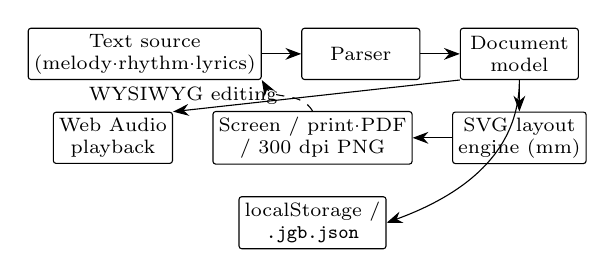
\begin{tikzpicture}[
  node distance=4mm and 5mm, font=\scriptsize,
  box/.style={draw, rounded corners=1pt, minimum height=6.5mm,
              minimum width=15mm, align=center, inner sep=2pt},
  arr/.style={-{Stealth[length=2mm]}}
]
  \node[box] (src) {Text source\\(melody·rhythm·lyrics)};
  \node[box, right=of src] (parser) {Parser};
  \node[box, right=of parser] (model) {Document\\model};
  \node[box, below=of model] (layout) {SVG layout\\engine (mm)};
  \node[box, left=of layout] (out) {Screen / print·PDF\\/ 300 dpi PNG};
  \node[box, left=of out] (audio) {Web Audio\\playback};
  \node[box, below=of out] (store) {localStorage /\\ \code{.jgb.json}};
  \draw[arr] (src) -- (parser);
  \draw[arr] (parser) -- (model);
  \draw[arr] (model) -- (layout);
  \draw[arr] (layout) -- (out);
  \draw[arr] (model.south west) -- (audio.north east);
  \draw[arr] (model.south) to[out=-90,in=20] (store.east);
  \draw[arr, dashed] (out.north) to[out=120,in=-60]
    node[midway, left, font=\scriptsize]{WYSIWYG editing} (src.south east);
\end{tikzpicture}
\caption{시스템 파이프라인. 텍스트 소스가 단일 원천이며, WYSIWYG 편집도
텍스트 갱신을 거쳐 동일 경로로 렌더링된다.\\
Fig.~\thefigure. System pipeline. The text source is the single source of
truth; WYSIWYG edits are also rendered through the same path via text
updates.}
\label{fig:arch}
\end{figure}

시스템은 \code{index.html}(마크업), \code{app.js}(로직, 약 4{,}100행),
\code{styles.css}(스타일)의 정적 파일 3개와, 율명 이미지·시김새 59종 SVG·
장구 구음 7종을 base64 데이터 URL로 내장한 데이터 파일 3개로 구성된다.
외부 라이브러리·서버·데이터베이스 의존이 전혀 없어 파일을 여는 것만으로
오프라인에서도 동작하며, 정적 호스팅(GitHub Pages)으로 배포된다.
이 구성은 교육 현장(설치 권한이 없는 공용 PC)과 장기 보존(플랫폼 종속성
최소화) 요구를 겨냥한 설계 결정이다.

그림~\ref{fig:arch}처럼 모든 편집은 텍스트 소스의 갱신으로 수렴하고,
파서가 이를 문서 모델로 해석하면 레이아웃 엔진이 SVG를 다시 그린다.
WYSIWYG 조작(입력 카드, 팔레트 클릭)도 내부적으로는 해당 정간의 텍스트
구간을 치환하는 것이므로, 두 입력 방식 사이에 표현 격차가 생기지 않는다.

\subsection{SVG 조판 엔진}

레이아웃은 A4 지면을 기준으로 물리 단위(mm)로 계산된다. 사용자는
한 각의 정간 수(1--64)·대강 분절·총 각 수·한 줄의 각 수·페이지당 줄 수·
정간 폭(4--30 mm)·각 간격·열 간격·머리단 등을 조정하고, 설정이 A4 인쇄
영역을 넘으면 비율을 유지한 채 자동 축소하고 축소율을 표시한다.
각은 전통 관행대로 오른쪽에서 왼쪽으로 흐르고, 대강은 프리셋
(10박=7·3, 12박=3·3·3·3, 16박=3·2·3·3·2·3, 20박=6·4·4·6) 또는 임의
분절로 굵은 선이 그어진다. 제목은 첫 페이지 오른쪽의 세로 칸(전통식)
또는 상단 가로줄로 배치할 수 있으며, 붓글씨체 등 서체·크기·자간을
지정할 수 있다. 화면 표시용 SVG와 인쇄·PNG용 SVG가 동일한 조판 결과를
공유하므로 ``보는 대로 인쇄된다''. 그림~\ref{fig:page}는 본 엔진이
조판한 A4 한 페이지의 300 dpi PNG 출력 전체이다.

\begin{figure}[t]
\centering
\fbox{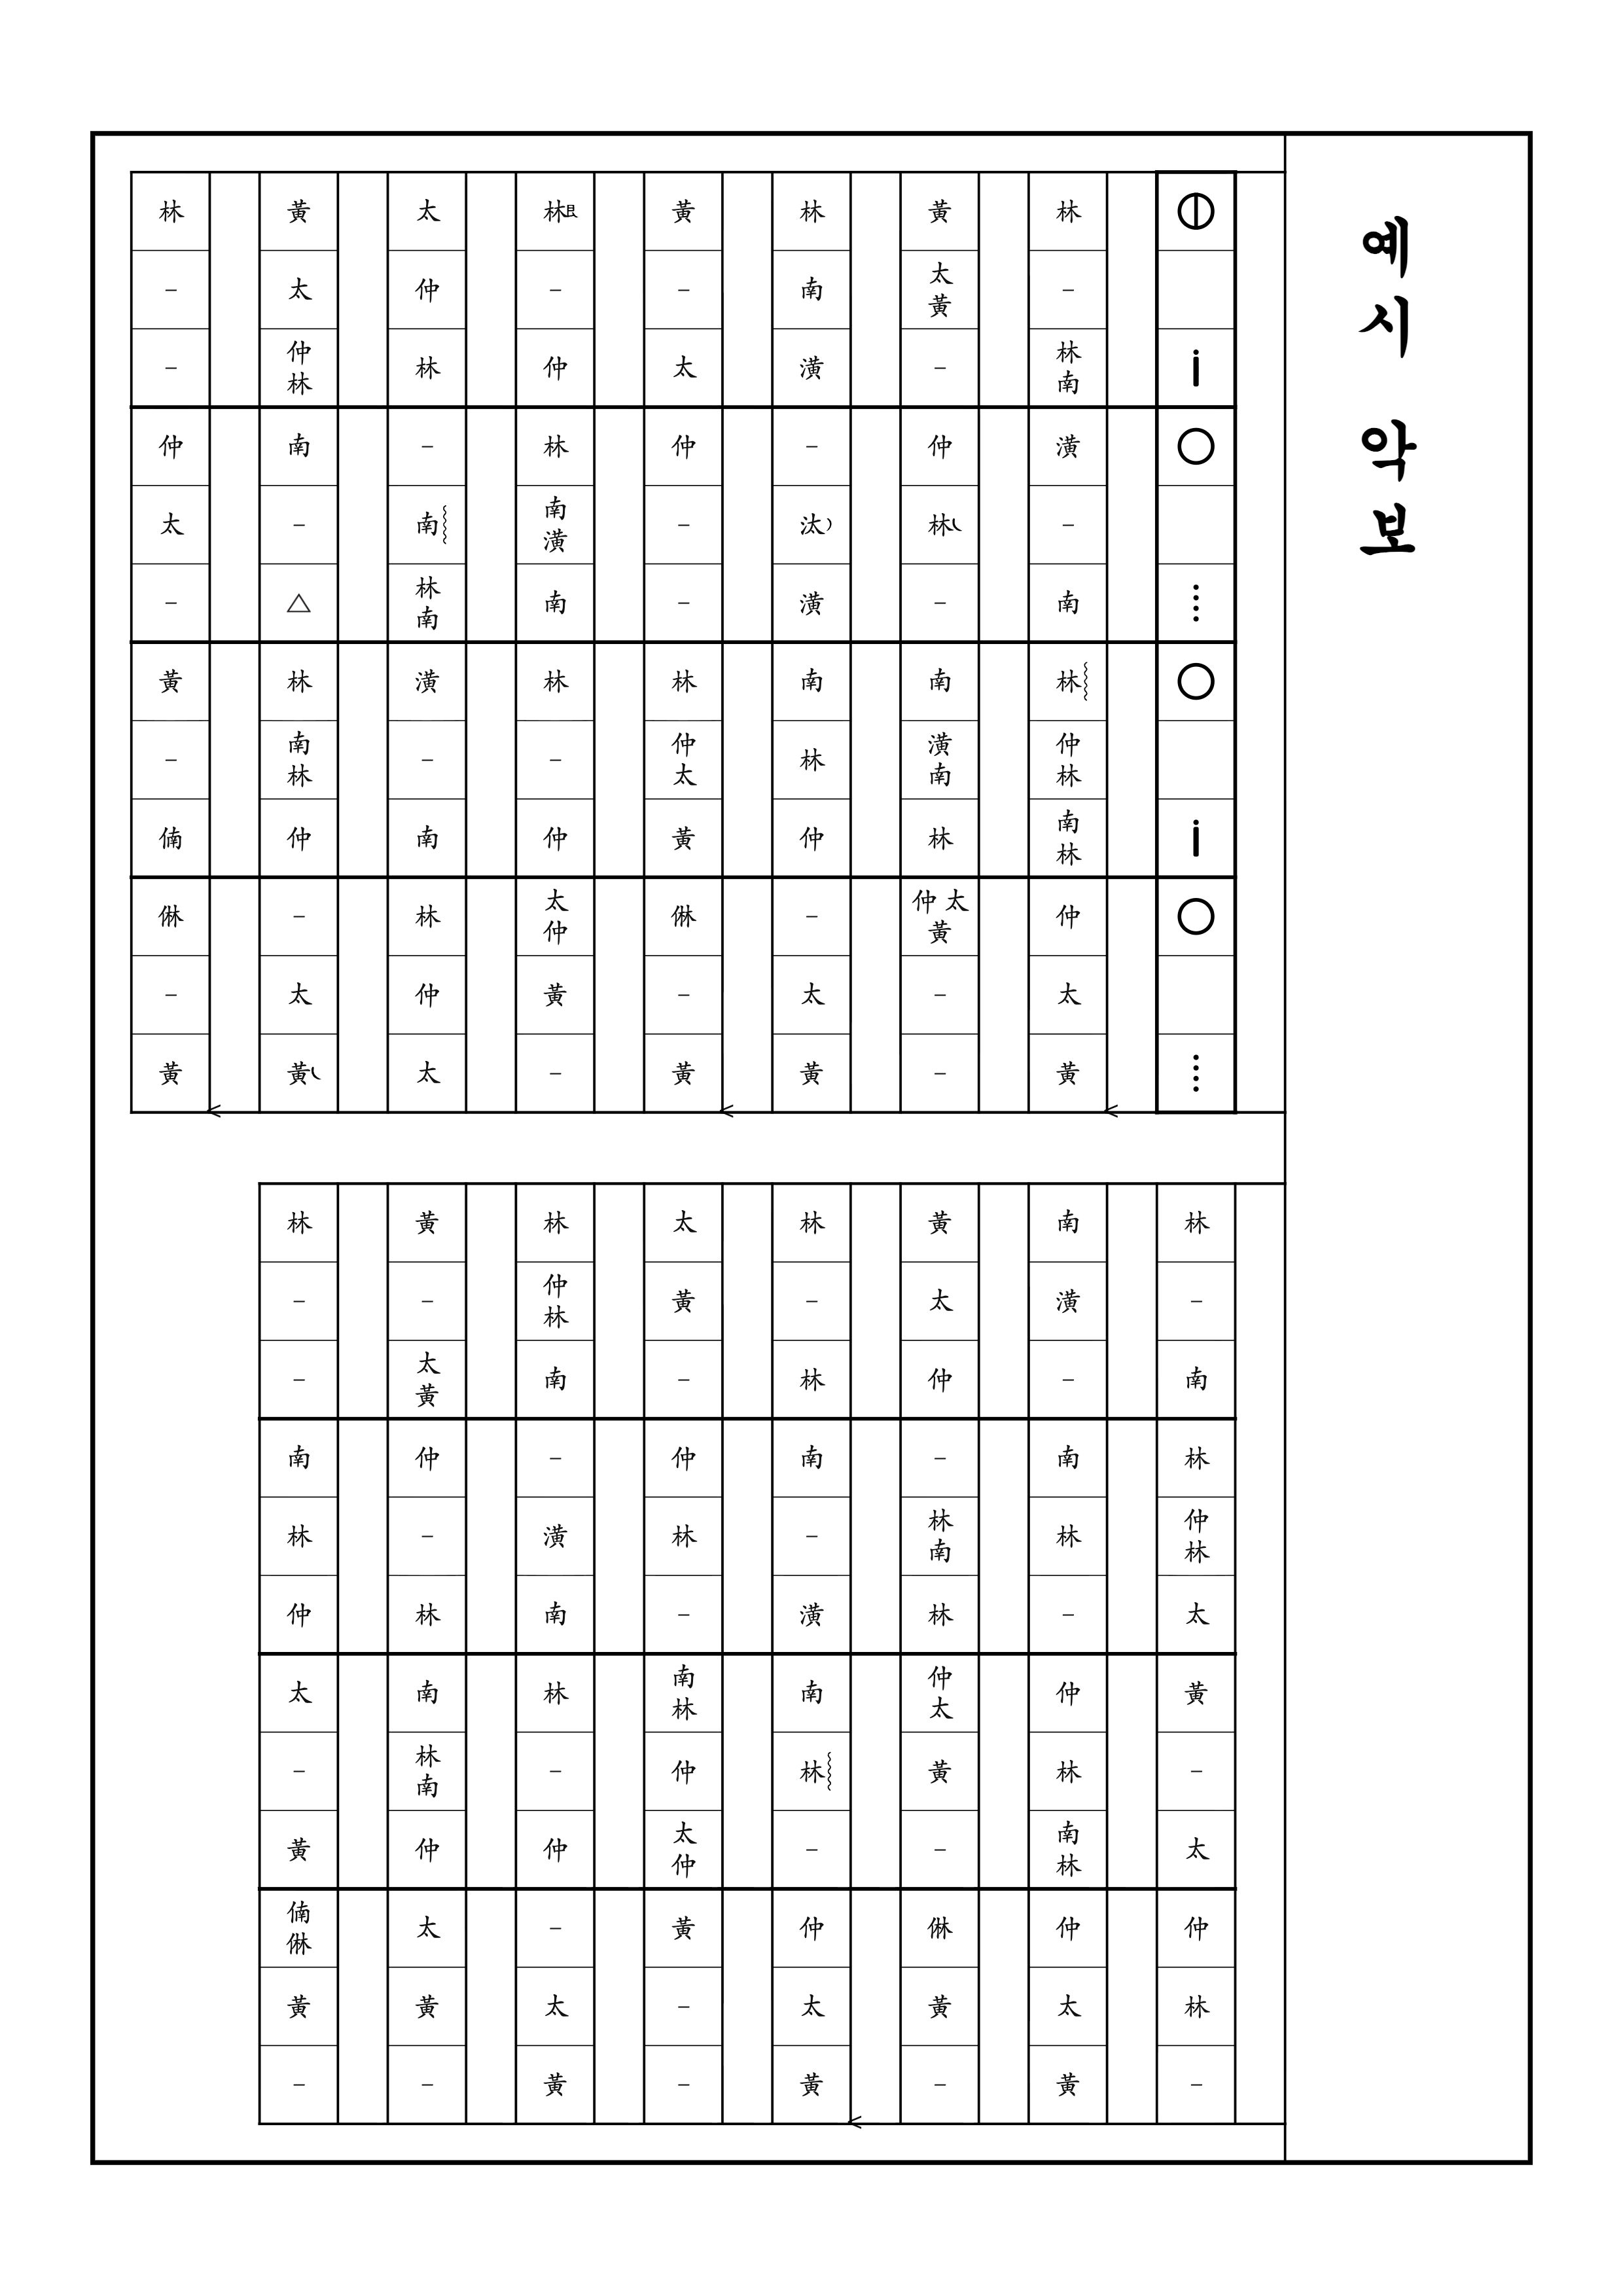
\includegraphics[width=0.86\columnwidth]{figures/fig-page.png}}

{\raggedright\scriptsize *Hangul/Hanja inside the figure is the score
content itself: jeongganbo notates pitches with Korean yulmyeong
characters.\par}
\caption{조판 결과 예 --- A4 세로, 12정간(대강 3·3·3·3), 한 줄 11칸
배치(세로 제목 칸 2 + 장단 각 1 + 선율 8각), 두 줄. 장단 각(맨 오른쪽
열)은 굵은 테두리로 선율 각과 구분되며, 각은 오른쪽에서 왼쪽으로
진행한다. 300 dpi PNG 내보내기 원본.\\
Fig.~\thefigure. Engraving example --- A4 portrait, 12 jeonggan per gak
(daegang 3·3·3·3), 11 columns per band (2 for the vertical title, 1 rhythm
gak, 8 melody gaks), two bands. The rhythm gak (rightmost column) is
distinguished by a thicker border, and gaks flow from right to left.
Original 300 dpi PNG export.}
\label{fig:page}
\end{figure}

\subsection{이중 입력과 양방향 동기화}

\textbf{직접 입력(WYSIWYG, 그림~\ref{fig:ui}).} 악보의 정간을 클릭하면
그 자리에 입력 카드가 열려 보이는 그대로 입력한다. Enter/Tab으로 다음 정간, 방향키로 인접 정간을
이동하며, 율명 팔레트(음역$\times$12율 매트릭스 또는 피아노 건반 뷰)와
시김새·장단 팔레트를 클릭해 채운다. 붙임표 시김새에는 숫자 단축키(1--0)가
배지로 표시되어, 숫자키로 고른 뒤 음을 클릭하면 즉시 부가된다.
문법을 전혀 몰라도 완전한 악보를 만들 수 있는 경로다.

\textbf{에디터(그림~\ref{fig:editor}).} 곡 전체를 텍스트로 편집한다.
각 정간 뒤에 탭을 자동 삽입해 줄이 달라도 \code{|}가 세로로 정렬되는
그리드 정렬, 해석 불가능한
토큰의 실시간 오류 표시(문법 검사), 여러 페이지 곡의 페이지 단위 표시를
제공한다. 반복 구절 복사·붙여넣기와 대량 수정에 강하다.

두 모드는 언제든 전환 가능하며, 악보에서 정간을 클릭하면 에디터의 해당
칸으로 커서가 이동하고 현재 칸이 악보에 하이라이트되는 양방향 동기화를
구현했다. 한글 입력기(IME; input method editor) 조합 중 keydown이
중복 발생하는 문제는
\code{isComposing} 가드로 처리했다.

\subsection{시김새 렌더링과 미세 조정}

시김새는 국립국악원 표기 관행을 기준으로 59종을 벡터화했다:
음표 오른쪽에 작게 붙는 붙임표 39종(미는표·흘림표·농음표 등),
한 칸을 차지하는 독립 기호 18종(전성·자출 등), 그리고 붙임·독립 양쪽으로
쓰이는 퇴성·추성 2종이다. 미세 조정 모드에서는 악보 위 시김새를 직접
클릭해 크기(40--300 \%)·좌우·상하(각 $\pm$90 \%)를 조정하고, 그 값은 3-3절의
문법으로 텍스트에 저장된다. 시김새 크기는 율명 크기 배율(0.7--2.5$\times$)과
독립적이어서 음표만 키워도 장식 기호의 균형이 유지된다.

\subsection{전통 조판 관행의 규칙화}

숙련 필사자의 지면 관행을 관찰하여 다음 규칙들을 렌더링 엔진에 명문화했다.
관찰 기준은 국립국악원 발간 악보(취타·군악 등)의 지면이다.
\TODO{기준으로 삼은 악보의 정확한 서지(간행물명·연도)를 명시하고
참고문헌에 추가할 것 --- 각주 금지 규정에 따라 본문·참고문헌으로 처리}

\begin{itemize}
  \item \textbf{이음(-) 축약}: 분박 여러 행 중 \code{-}만 홀로 있는 행은
        세로 비중을 0.68로 줄이고 남는 공간을 음표 행에 배분하여,
        지속 기호가 실제 음처럼 크게 보이지 않게 한다. \code{-} 글리프는
        가로로 1.95배 늘여 짧아 보이지 않게 하고 세로 중심을 보정한다.
  \item \textbf{2음 간격 압축}: 정간에 음이 정확히 둘이면(세로 분박이든
        가로 붙임이든) 간격을 20 \% 좁혀 성긴 인상을 막는다.
  \item \textbf{옥타브 변형 한자 우선}: 한자 모드에서는 潢(청황) 등
        변형자를 우선 쓰고, 변형자가 없는 조합에만 기본 한자에 옥타브 점을
        병기한다($\pm2$옥타브 지원). 한글 모드에서는 2글자 68 \%,
        3글자 50 \%로 자동 축소하여 칸을 넘지 않는다.
  \item \textbf{계층별 시각 구분}: 장단 각은 일반 각보다 굵은 테두리로
        둘러 선율 각과 구분하고, 반복 패턴인 장단은 곡 첫 각 옆에
        한 번만 표시한다.
\end{itemize}

\begin{figure}[t]
\centering
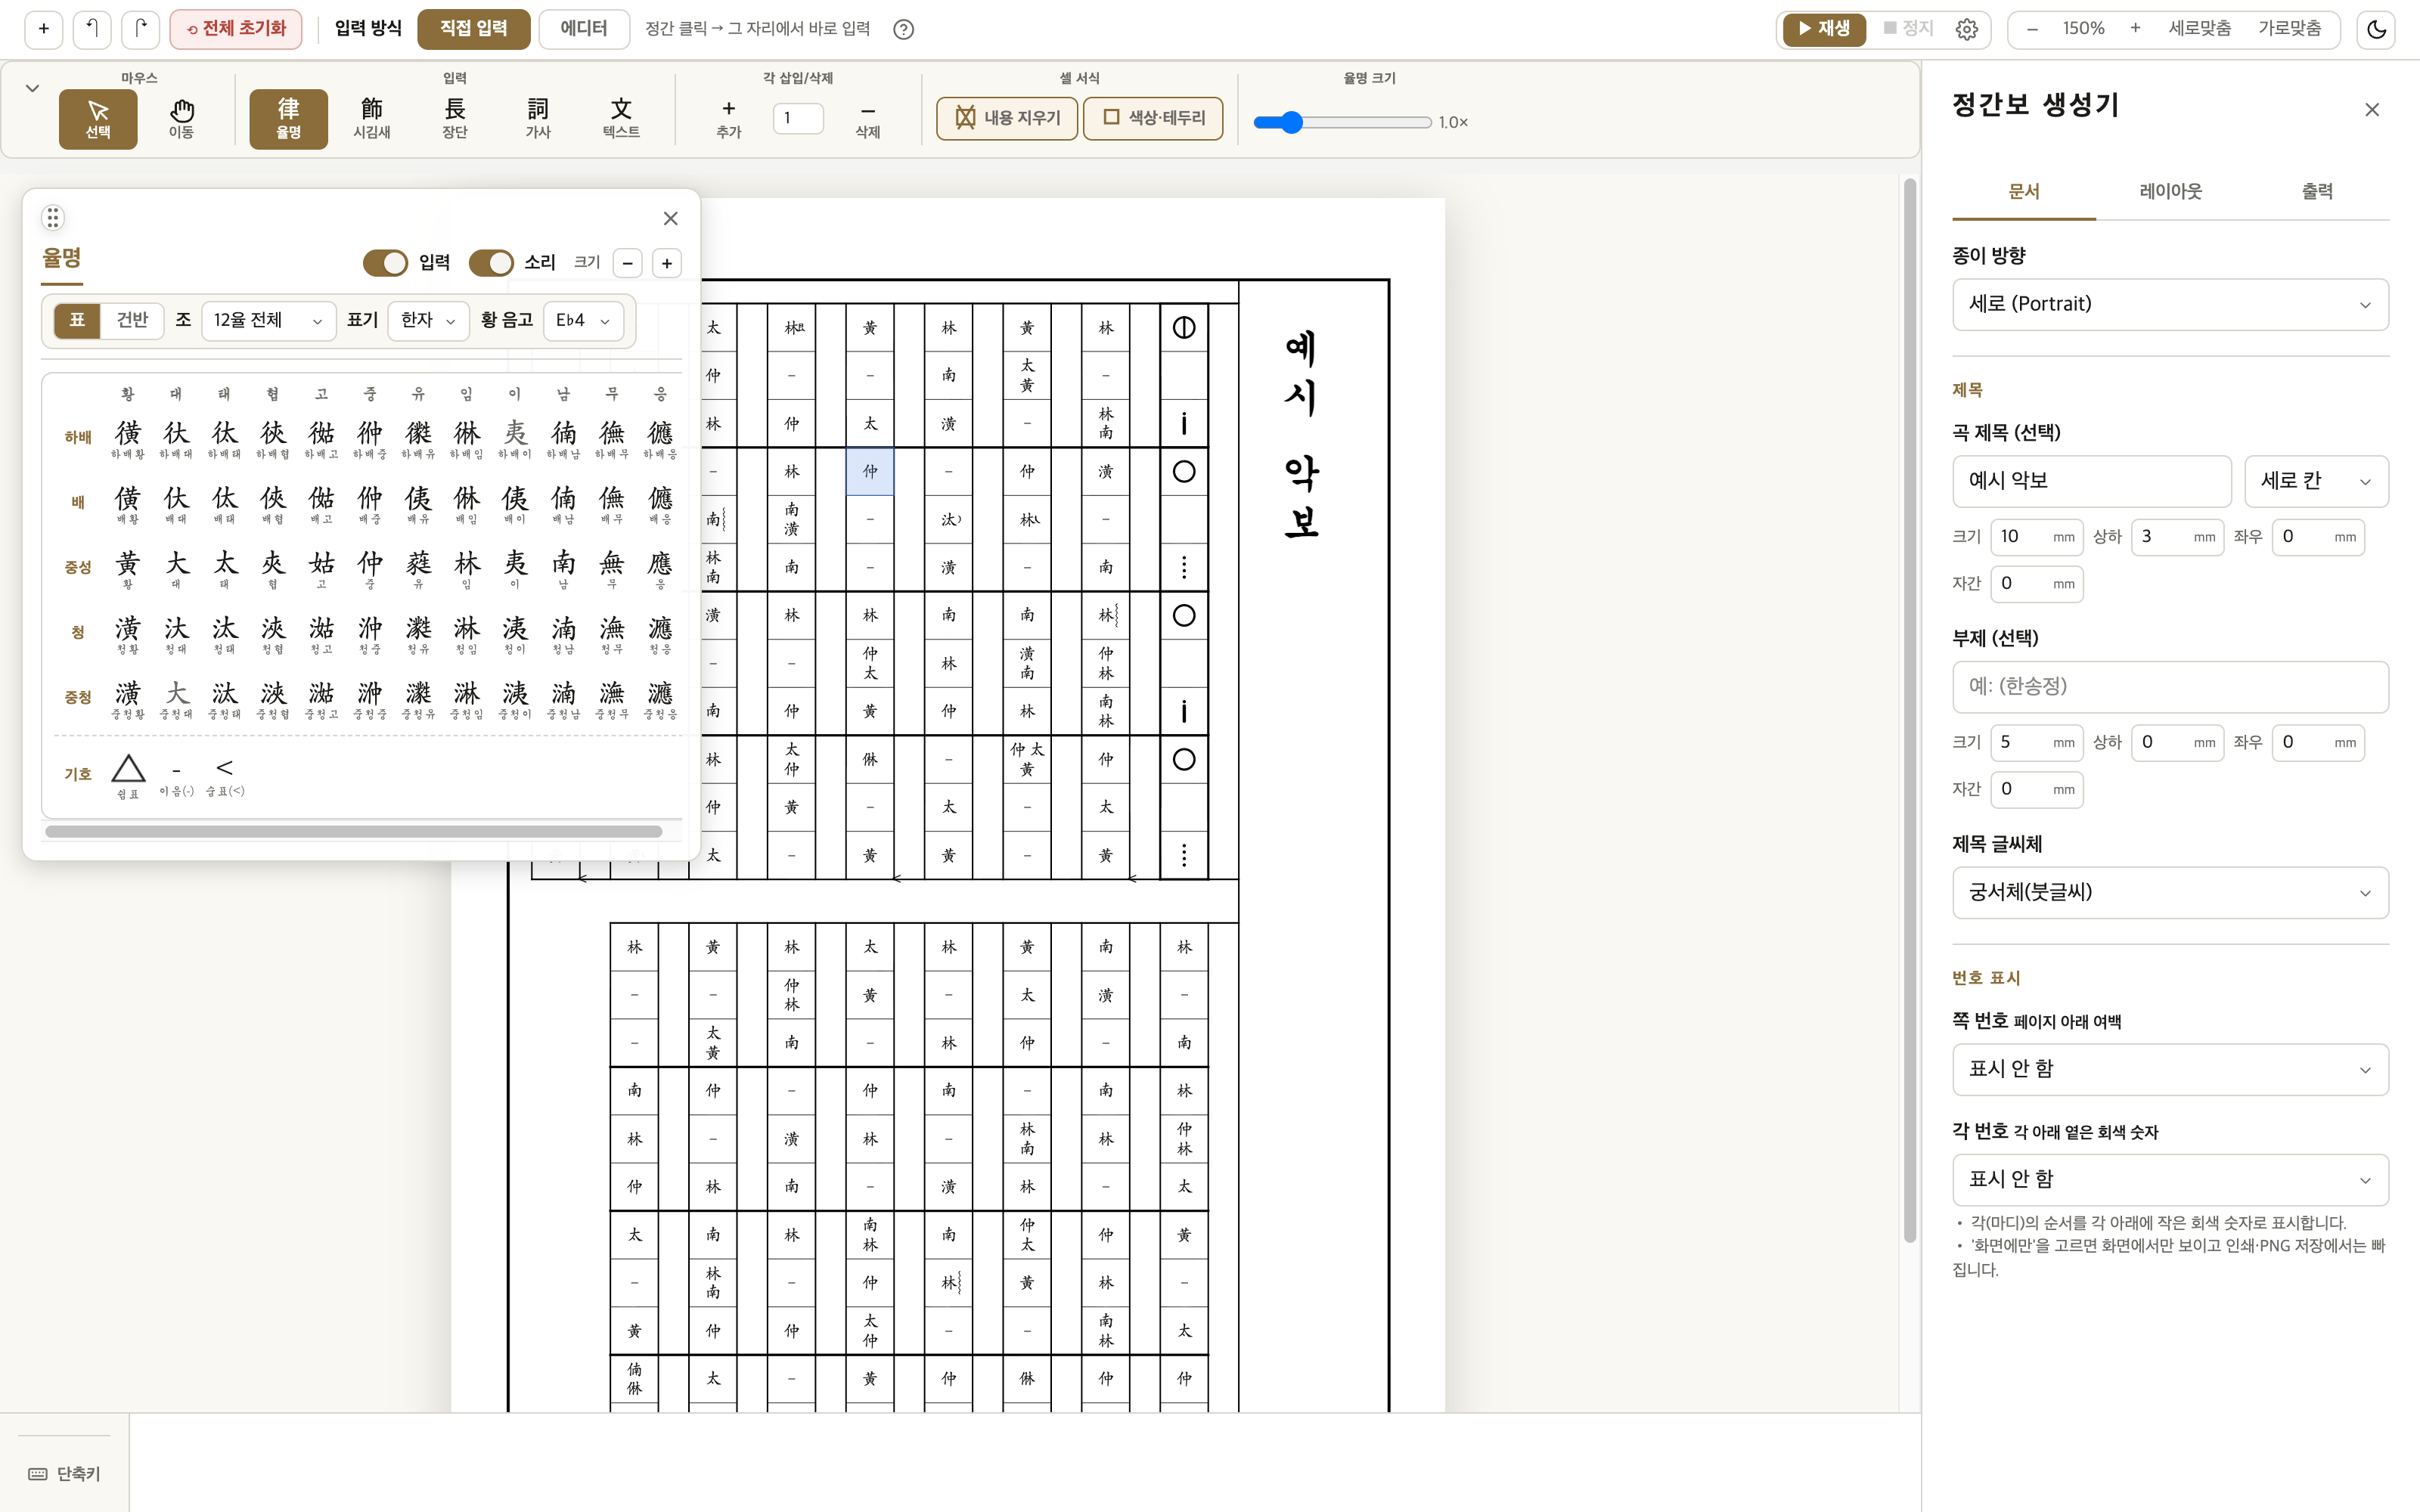
\includegraphics[width=\columnwidth]{figures/fig-ui.png}

{\raggedright\scriptsize *The UI is in Korean because the target users are
Korean traditional music practitioners; the score content itself also uses
Korean pitch-name characters.\par}
\caption{직접 입력 모드 편집 화면. 율명 도구창(음역$\times$12율 매트릭스,
한자·한글 병기)이 악보 위에 떠 있고, 클릭한 정간(파란 하이라이트)에
팔레트 선택이 바로 입력된다. 오른쪽은 문서 설정 사이드바.\\
Fig.~\thefigure. Editing screen in direct-input mode. The pitch-name
palette (register $\times$ 12 pitches, Hanja/Hangul) floats over the score;
a palette click fills the highlighted (blue) cell. The document settings
sidebar is on the right.}
\label{fig:ui}
\end{figure}

\begin{figure}[t]
\centering
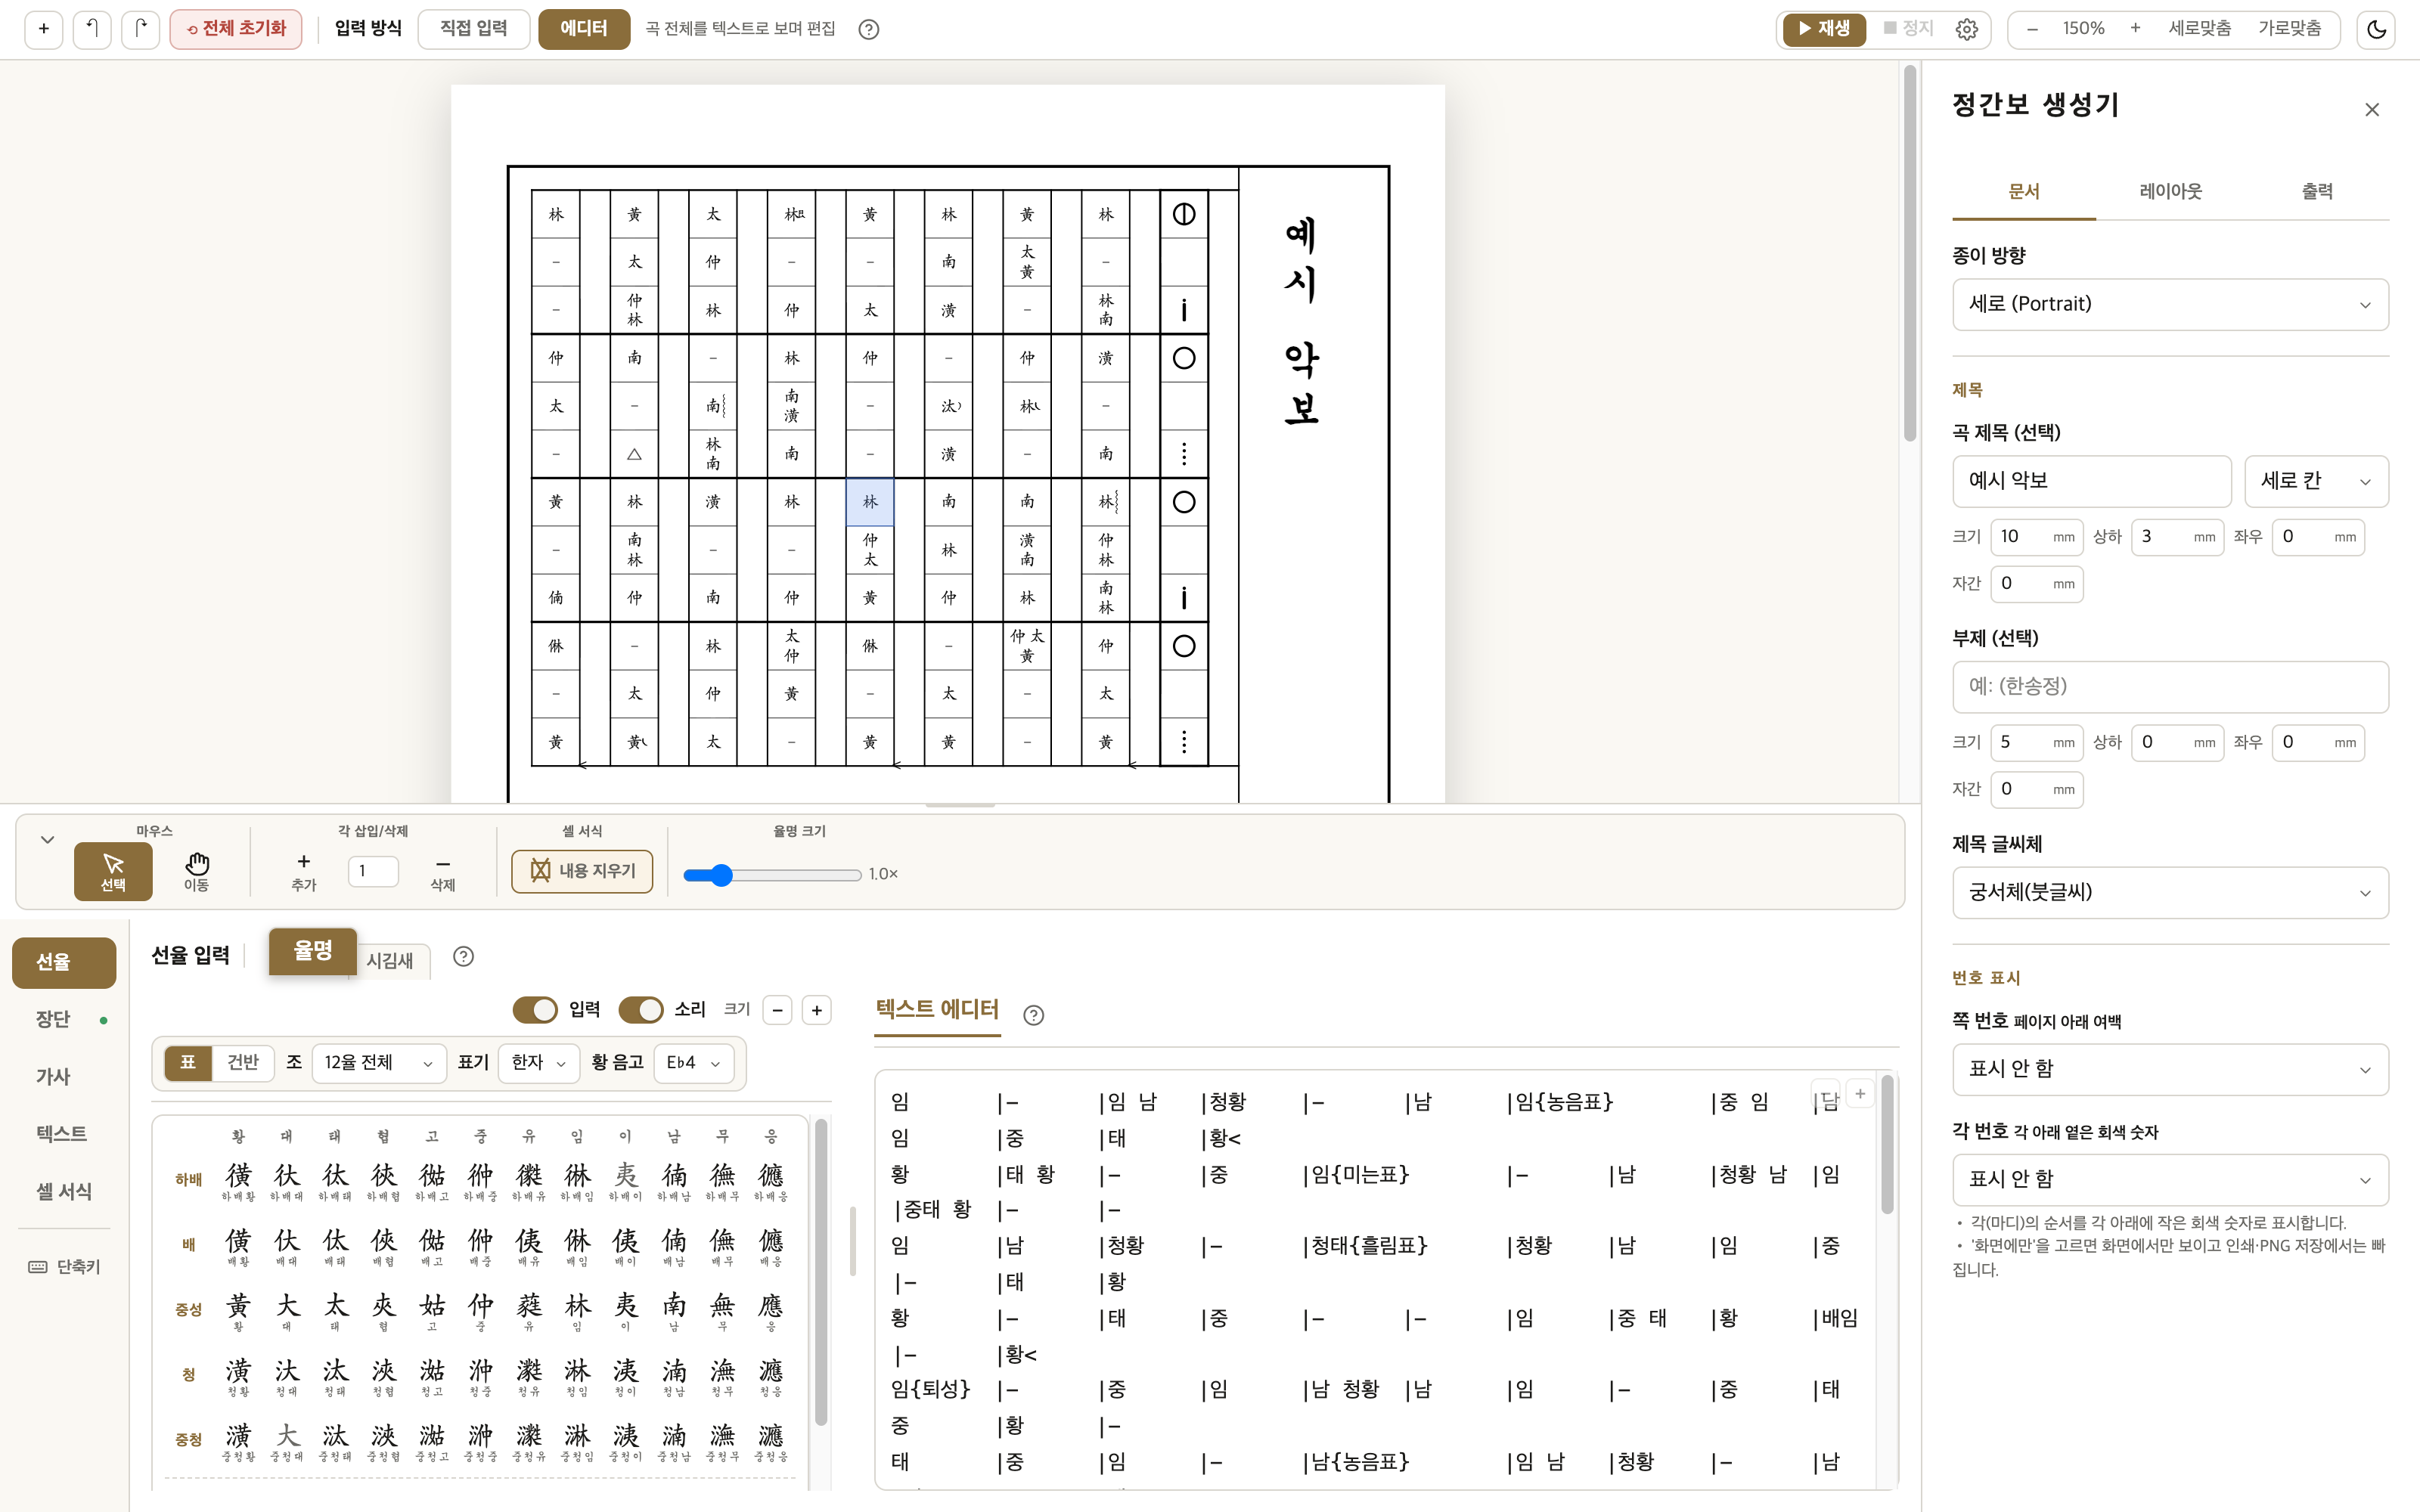
\includegraphics[width=\columnwidth]{figures/fig-editor.png}

{\raggedright\scriptsize *The UI and score content are in Korean; see the
note of Fig.~\ref{fig:ui}.\par}
\caption{에디터 모드. 아래 편집 독의 텍스트 에디터는 정간 구분자
\code{|}가 세로로 정렬되는 그리드 정렬을 제공하며, 악보에서 정간을
클릭하면 에디터의 해당 위치로 커서가 이동하고 그 정간이 악보에
하이라이트된다(양방향 동기화).\\
Fig.~\thefigure. Editor mode. The text editor in the bottom dock aligns
jeonggan separators \code{|} vertically (grid alignment); clicking a cell
in the score moves the cursor to the corresponding token and highlights
the cell (two-way synchronization).}
\label{fig:editor}
\end{figure}

\begin{figure*}[t]
\centering
\begin{minipage}[c]{0.56\textwidth}
\scriptsize
\begin{verbatim}
임|-|임 남|청황|-|남|임{농음표}|중 임|남 임|중|태|황<
황|태 황|-|중|임{미는표}|-|남|청황 남|임|중태 황|-|-
임|남|청황|-|청태{흘림표}|청황|남|임|중|-|태|황
\end{verbatim}
\end{minipage}\hfill
\begin{minipage}[c]{0.40\textwidth}
\centering
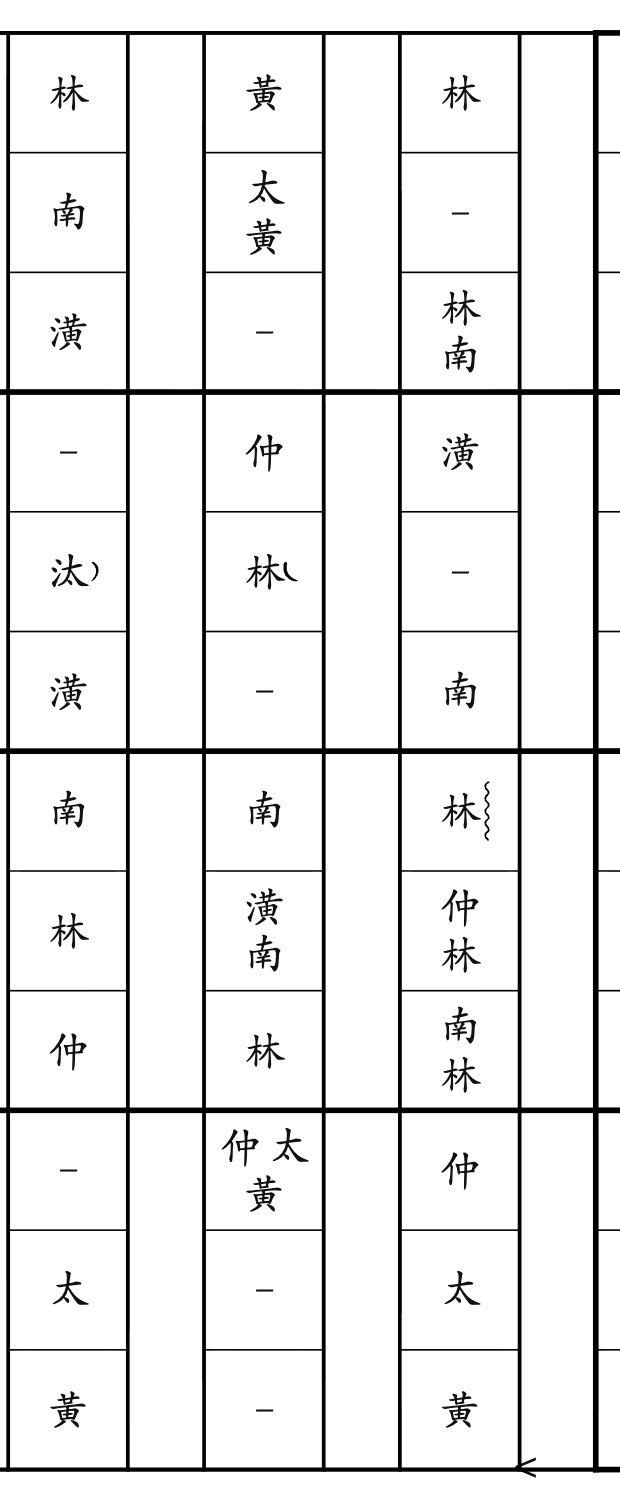
\includegraphics[height=88mm]{figures/fig-mapping.png}
\end{minipage}

{\raggedright\scriptsize *Korean characters here are the notation input
and output themselves (pitch names and ornament names).\par}
\caption{텍스트 문법(왼쪽)과 조판 결과(오른쪽)의 대응. 텍스트 첫 행이
오른쪽 그림의 맨 오른쪽 각에 해당한다(우종서). \code{|}가 정간 경계,
공백이 분박(예: 1행 셋째 정간 \code{임 남}), 연접이 붙임(2행
\code{중태 황}), \code{-}가 이음, \code{<}가 숨표로 대응되고,
시김새 \code{\{농음표\}} 등은 음표 곁의 기호로 그려진다.
굵은 가로선은 대강(3·3·3·3) 경계이다.\\
Fig.~\thefigure. Correspondence between the text grammar (left) and the
engraved result (right). The first text line maps to the rightmost gak
(right-to-left order). \code{|} marks jeonggan boundaries, spaces mark
subdivisions (e.g., \code{임 남} in line 1), juxtaposition marks horizontal
grouping (\code{중태 황} in line 2), \code{-} marks sustain, \code{<} marks
a breath, and \code{\{...\}} attaches ornaments. Thick horizontal lines are
daegang (3·3·3·3) boundaries.}
\label{fig:mapping}
\end{figure*}

\subsection{셀 서식과 편집 지원}

교육 자료 제작을 위해 정간 단위의 배경색과 변(邊) 단위 테두리
(전체/바깥쪽/안쪽 프리셋, 변 개별 선택, 3단계 굵기, 실선·점선·이중선·없음)를
지원한다. `없음'은 해당 위치의 원래 정간선까지 숨기되 악보 뼈대인 통줄과
대강선은 보호한다. 실행 취소는 문서 내용 변경만을 스냅샷(600 ms 디바운스)으로
쌓는 전역 단일 스택(Cmd/Ctrl+Z)으로 통일하여, 장단·가사 초기화나 임시 저장
불러오기까지 모두 복구된다. 다크 모드에서는 UI만 어두워지고 악보 지면은
항상 흰색을 유지해 인쇄·PNG 출력이 화면 테마와 무관하게 일정하다.

\subsection{재생}

Web Audio API로 사인파 합성 재생을 제공한다. 정간 1칸 = 1박, 분박은 등분,
빈 정간과 이음은 앞 음을 지속하며 쉼표만 무음으로 처리한다.
기준 음고는 황종 = E$\flat$4(전통 기준) 또는 C4를 선택할 수 있고
템포는 20--240 BPM(beats per minute)이다. 템포 표시를 켜면 첫 각 위에
``一分·六十井''(1분에 60정간)처럼 한자 세로 표기가 부가되는데, 이는
분당 정간 수로 빠르기를 적는 국악보 관행을 따른 것이다. 재생 중 현재
정간이 악보에 하이라이트되어 초심자의 독보(讀譜) 학습을 돕는다.

\subsection{저장과 문서 교환}

저장은 3단계다. (1) 모든 입력이 브라우저 \code{localStorage}에 즉시
자동 저장되고, (2) 이름 붙인 임시 저장 슬롯으로 여러 버전을 보관하며,
(3) 문서 전체(레이아웃 설정+선율+장단+가사+자유 텍스트+셀 서식)를
\code{.jgb.json} 파일로 내보내고 불러온다. JSON 컨테이너 안에 Ⅲ장의
텍스트 문법이 그대로 담기므로 파일은 사람이 열어 읽을 수 있고,
OMR~\cite{kim2025omr} 등 외부 파이프라인의 출력 포맷으로 쓰기에도 용이하다.
인쇄(브라우저 인쇄 대화상자를 통한 PDF 포함)와 페이지별 300 dpi PNG
다운로드를 지원한다.

\section{결과 및 논의}
\label{sec:discussion}

\subsection{기존 도구·연구와의 기능 비교}

\begin{table*}[t]
\centering\small
\caption{정간보 관련 도구·연구와의 기능 비교
(\(\bullet\)=지원, \(\circ\)=부분 지원, ---=미지원)}
\label{tab:compare}
\begin{tabular}{@{}lcccccc@{}}
\toprule
 & 본 시스템 & XML 기술~\cite{lee2013xml} & 웹 설계~\cite{jkca2022web}
 & 웹 편집기~\cite{jeongganbo-editor-web} & HWP 표 조판 & MuseScore~\cite{musescore} \\
\midrule
사람이 읽는 텍스트 문법      & \(\bullet\) & --- & --- & --- & --- & --- \\
WYSIWYG 편집                & \(\bullet\) & --- & \(\circ\) & \(\bullet\) & \(\bullet\) & \(\bullet\) \\
분박·붙임(위치 시가)         & \(\bullet\) & \(\bullet\) & \TODO{확인} & \(\circ\) & \(\circ\) & --- \\
시김새                      & \(\bullet\)(59종) & \(\circ\) & \TODO{확인} & --- & \(\circ\)(수작업) & --- \\
장단·가사 계층               & \(\bullet\) & \(\circ\) & \TODO{확인} & --- & \(\circ\)(수작업) & --- \\
우종서·대강 조판             & \(\bullet\) & \(\circ\) & \TODO{확인} & \(\circ\) & \(\circ\)(수작업) & --- \\
재생                        & \(\bullet\) & \(\circ\) & --- & --- & --- & \(\bullet\)(오선보) \\
인쇄·PDF·PNG 출력            & \(\bullet\) & --- & --- & \(\circ\)(PNG) & \(\bullet\) & \(\bullet\) \\
구조화 문서 교환             & \(\bullet\)(JSON) & \(\bullet\)(XML) & \TODO{확인} & \(\circ\)(JSON) & --- & \(\bullet\)(MusicXML) \\
서버리스·오프라인            & \(\bullet\) & 해당 없음 & \TODO{확인} & --- & \(\bullet\) & \(\bullet\) \\
\bottomrule
\end{tabular}
\end{table*}

표~\ref{tab:compare}에 정간보 관련 도구·연구와의 기능 비교를 정리했다.
본 시스템은 텍스트 문법과 WYSIWYG을 겸비하고 시김새·장단·가사·조판·출력·
재생을 한 도구에서 지원한다는 점에서, 인코딩 제안에 머문 연구나 기본
격자 입력만 제공하는 기존 편집기와 구별된다.
\TODO{비교표의 각 칸을 해당 도구를 직접 실행/원문 확인 후 재검증할 것 ---
특히 jkca2022web 열은 현재 추정임}

\subsection{사례 연구: 간행 악보 재현}

본문 그림들(그림~\ref{fig:ui}--\ref{fig:mapping})의 문서는 문법 요소를
고루 포함하도록 구성한 예시 악보이다. 간행 악보 재현의 사례 연구로는
해금정악보의 군악(12정간, 대강 3·3·3·3)을 대상으로 원본 지면과 동일한
배치(세로 제목 칸·장단 열·시김새 포함)를 재현하고 원본 스캔과 나란히
비교할 계획이다.
\TODO{저자 직접 작업 필요: `악보 예시/예시 이미지-12박(대강3333).png'
(해금정악보 68쪽 군악)를 채보해 재현하고 --- 해금 활대 방향 표시 등
관악보 고유 기호의 처리 방식 결정 포함 --- 원본/출력 비교 그림, 입력
소요 시간, 텍스트 소스 길이, \code{.jgb.json} 파일 크기 등 정량 정보를
기입할 것. 원본 스캔 게재 시 저작권 확인 필요}
전 과정에 서버 통신이 없고, 완성 문서는 수십 KB 수준의
\code{.jgb.json} 하나로 보존·공유된다.

\subsection{한계}

현재 구현의 한계는 다음과 같다.
첫째, 재생이 사인파 단선율에 그치며 시김새·장단이 소리에 반영되지 않는다.
시김새는 본질적으로 미분음적 음높이 굴곡이므로, 기호별 음고 궤적
모델링이 필요하다.
둘째, 셀 서식(배경색·테두리)이 선율 정간에만 적용되고 장단·가사 칸은
지원하지 않는다.
셋째, MusicXML·MEI 등 표준 포맷과의 상호 변환이 없어 오선보 병기나
서양 도구 연계가 수동이다.
넷째, 사용성 평가를 아직 수행하지 않았다. 국악 전공자·교사를 대상으로
과제 기반 평가(기존 HWP 조판 대비 작성 시간·오류율·SUS 점수)를 수행하는
것이 후속 과제다. \TODO{투고 전 소규모라도 사용자 평가를 실시해 5장을
평가 결과 중심으로 재구성하는 것을 강력 권장 --- JDCS 심사에서 평가 부재가
지적될 가능성이 높음}

\section{결론 및 향후 연구}
\label{sec:conclusion}

본 논문은 정간보의 격자 구조를 텍스트에 그대로 옮긴 경량 문법과, 이를
단일 원천으로 삼는 서버리스 웹 편집·조판 시스템 ``정간보 생성기''를
제안했다. 시스템은 WYSIWYG과 텍스트 편집의 양방향 동기화, 시김새 59종의
벡터 렌더링과 텍스트 직렬화, 전통 조판 관행의 규칙화, mm 단위 SVG 조판을
통한 인쇄·PDF·PNG 출력, JSON 문서 교환, Web Audio 재생을 정적 파일만으로
구현하여, 워드프로세서 수작업에 머물러 있던 정간보 제작을 데이터 기반
워크플로로 전환할 수 있음을 보였다.

향후 연구는 세 방향이다.
첫째, \textbf{소니피케이션 고도화}: 시김새의 음고 궤적과 장단 타점을
합성에 반영하고, 산조·정악 등 장르별 음색 모델을 얹어 ``들리는 정간보''로
확장한다.
둘째, \textbf{상호운용성}: \code{.jgb.json}과 MEI/MusicXML 간 변환기를
구현해 오선보 병기와 음악학 도구 연계를 지원하고, 정간보
OMR~\cite{kim2025omr} 출력의 표준 컨테이너로 문법을 제안한다.
이는 세종실록악보 등 고악보 아카이브~\cite{han2024sixdragons}를
편집 가능한 형태로 되살리는 파이프라인의 마지막 조각이 된다.
셋째, \textbf{사용자 연구}: 국악 교육 현장 투입을 통한 과제 기반 사용성
평가와 교육 효과 검증을 수행한다.

시스템은 오픈 웹에 공개되어 있다.
\TODO{배포 URL·저장소 공개 여부 결정 후 기입 (GitHub Pages 주소)}

% ------------------------------------------------------------
\section*{감사의 글}
\TODO{연구비 지원·사사 문구 (해당 시)}


% ------------------------------------------------------------
% 참고문헌 — JDCS 규정:
%   · 반드시 영문 표기(국문 문헌도 영문으로), 본문 인용 순서대로 번호
%   · 논문지: 저자, "제목," 논문지명, Vol., No., pp., 월 년. doi
%   · 모든 단어 첫 글자 대문자, URL은 하이퍼링크 해제
%   · 본문에 인용된 것만 수록(미인용 항목 금지)
% ieeetr 자동 생성으로는 이 형식이 안 나와 수동 목록으로 전환했다.
% 서지 원천 데이터는 references.bib에 계속 유지(TODO 목록 포함).
% ------------------------------------------------------------
\begin{thebibliography}{99}\small

\bibitem{kwon2000notation}
O. S. Kwon, \textit{History of Korean Notations}, \TODO{출판사·소재지},
2000. \TODO{실제 인용 판본으로 서지 확정(대안: 장사훈 국악총론 등)}

\bibitem{han2024sixdragons}
D. Han, M. Gotham, D. Kim, H. Park, S. Lee, and D. Jeong,
``Six Dragons Fly Again: Reviving 15th-Century Korean Court Music with
Transformers and Novel Encoding,'' in \textit{Proceedings of the 25th
International Society for Music Information Retrieval Conference (ISMIR)},
San Francisco, CA, pp. 1--8, Nov. 2024. \TODO{최종 페이지 확인}

\bibitem{musescore}
MuseScore BVBA, \textit{MuseScore: Free Music Composition and Notation
Software} [Internet]. Available: https://musescore.org/. \TODO{버전 명시}

\bibitem{musescore-jgb-request}
MuseScore Community Forum, \textit{Jeongganbo Notation (Feature Request)}
[Internet]. Available: https://musescore.org/en/node/356508.

\bibitem{lee2013xml}
Y. J. Lee, ``A Study on the Musical Notation of Jeongganbo Using Extensible
Markup Language,'' \textit{The Journal of the Acoustical Society of Korea},
Vol. 32, No. 5, pp. 446--455, Sep. 2013.
https://doi.org/10.7776/ASK.2013.32.5.446
\TODO{영문 제목·공저자·DOI 원문 대조}

\bibitem{patent2017jgb}
Electronics and Telecommunications Research Institute, \textit{Method for
Describing Jeongganbo Music Score and Method for Playing Jeongganbo Music
Score}, Korean Patent KR101789851B1, Oct. 2017. \TODO{발명자 성명 확인}

\bibitem{jkca2022web}
\TODO{저자}, ``Designing a Web-Based Jeongganbo Notation Program,''
\textit{The Journal of the Korea Contents Association}, Vol. 22,
\TODO{No.·pp.·월}, 2022. \TODO{서지 전체 확인(KoreaScience JAKO202213253766158)}

\bibitem{kim2025omr}
\TODO{저자 명단(MALerLab)}, ``On the Automatic Recognition of Jeongganbo
Music Notation: Dataset and Approach,'' \textit{ACM Journal on Computing and
Cultural Heritage}, 2025. https://doi.org/10.1145/3715159
\TODO{권·호·페이지 확인}

\bibitem{jeongganbo-editor-web}
\textit{Jeongganbo Editor} [Internet]. Available: https://jeongganbo.com/.
\TODO{개발자·공개 연도 확인}

\bibitem{good2001musicxml}
M. Good, ``MusicXML: An Internet-Friendly Format for Sheet Music,'' in
\textit{Proceedings of XML 2001}, Orlando, FL, pp. 3--4, Dec. 2001.
\TODO{개최지·페이지 확인}

\bibitem{mei}
Music Encoding Initiative, \textit{MEI Guidelines} [Internet].
Available: https://music-encoding.org/. \TODO{인용 시점 버전 명시}

\bibitem{verovio}
L. Pugin, R. Zitellini, and P. Roland, ``Verovio: A Library for Engraving
MEI Music Notation into SVG,'' in \textit{Proceedings of the 15th
International Society for Music Information Retrieval Conference (ISMIR)},
Taipei, Taiwan, pp. 107--112, Oct. 2014.

\bibitem{abc}
C. Walshaw, \textit{The ABC Music Standard 2.1} [Internet].
Available: https://abcnotation.com/wiki/abc:standard:v2.1.

\bibitem{humdrum}
D. Huron, \textit{The Humdrum Toolkit: Reference Manual}, Center for
Computer Assisted Research in the Humanities, Menlo Park, CA, 1994.

\end{thebibliography}

% ------------------------------------------------------------
% 저자 약력 — 게재 확정본에만 넣는다(심사용 파일에서는 삭제).
% 형식: 이름(영문명) / 연도: 학력·경력 / ※관심분야: …
% 사진 28×29mm, 300dpi, jpg.
% ------------------------------------------------------------
% \section*{저자약력}
% \TODO{저자 약력·사진 (심사용 파일에는 넣지 않음)}

\end{document}
